\begin{frame}{Architecture Trends}
\begin{itemize}
\item Computing platforms are more and more complex
\item We classify them into four categories:
\begin{itemize}
\item Shared memory architectures
\item Distributed memory architectures
\item Hierarchical architectures
\item Heterogeneous architectures
\end{itemize}
\end{itemize}
\end{frame}

\begin{frame}{Programming Paradigm}
Historically, we use:
\begin{itemize}
\item Message passing (MPI) for distributed memory architectures
\item Threads library (OMP) for shared memory architectures
\item Accelerator library (OpenCL) for accelerator of heterogeneous architectures
\end{itemize}
\pause
$\Rightarrow$ Several programs for the same algorithm\\
$\Rightarrow$ Weak portability\\
$\Rightarrow$ Weak scalability\\
\pause
\begin{exampleblock}{Solution:}
Recent paradigm of programming which separate algorithm from architectures used: \textbf{Task Flow Model}
\end{exampleblock}
\end{frame}

\begin{frame}{Task Flow Model}
Programs can be represented by a Direct Acyclic Graph (DAG) where:
\begin{itemize}
\item Vertices are tasks
\item Edges are data dependencies between tasks
\end{itemize}
\pause
\begin{flushleft}
$\Rightarrow$ One single implementation of the DAG in a specific language
\end{flushleft}
\pause
\begin{flushleft}
Execution of tasks and data movement between them assured by the \textbf{Runtime}
\end{flushleft}
\end{frame}

\begin{frame}{Runtimes}
\begin{exampleblock}{Advantages :}
\begin{itemize}
\item Abstraction of architectures
\item Portability of performance
\item Good reactivity for load imbalance
\item Natural look ahead
\end{itemize}
\end{exampleblock}{}
\pause
\begin{exampleblock}{Challenge:}
At the moment, runtimes are efficient for model of architectures
\begin{itemize}
\item DAGuE for large hierarchical architectures
\item StarPU for heterogeneous architectures
\end{itemize}
\end{exampleblock}{}
\end{frame}

\subsection{$A=LU$}

\begin{frame}{Why LU decomposition}
In order to solve square systems of linear equations:
\begin{center}
$Ax=b$
\end{center}
Use LU decomposition (Gaussian elimination):
\begin{center}
$A=LU$
\end{center}
Where $L$ is a lower triangular matrix with the identity diagonal and $U$ an upper triangular matrix.

Then solve:
\begin{center}
$Ly=b$ then $Ux=y$
\end{center}
\end{frame}

\begin{frame}{LU algorithm}
\begin{columns}[c]
\begin{column}{0.02\textwidth}
\end{column}
\begin{column}{0.60\textwidth}
\begin{tabbing}
Let be $A$ a $n*n$ square matrix\\
For \= $k$ from $1$ to $n$\\
\> For \=$i$ from $k+1$ to $n$\\
\>\> \textcolor{red}{$a_{i,k} = a_{i,k}/a_{k,k}$}\\
\> For \=$i$ from $k+1$ to $n$\\
\>\> For \=$j$ from $k+1$ to $n$\\
\>\>\> \textcolor{borange}{$a_{i,j} = a_{i,j}-a_{i,k}*_{k,j}$}\\
\end{tabbing}
\end{column}
\begin{column}{0.02\textwidth}
\end{column}
\begin{column}{0.35\textwidth}
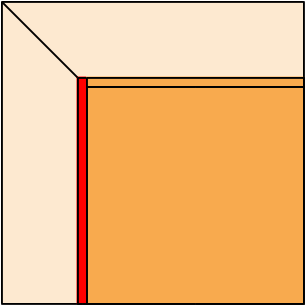
\includegraphics[width=0.8\linewidth]{linpack}
\end{column}
\end{columns}
\end{frame}

\subsection{$PA=LU$}
\begin{frame}{LU decomposition problem}
\begin{columns}[c]
\begin{column}{0.02\textwidth}
\end{column}
\begin{column}{0.45\textwidth}
\begin{tabbing}
Let be $A$ a $n*n$ square matrix\\
For \= $k$ from $1$ to $n$\\
\>\visible<3->{\alert{Search for pivot then swap}}\\
\> For \=$i$ from $k+1$ to $n$\\
\>\> $a_{i,k} = a_{i,k}/a_{k,k}$\\
\> For \=$i$ from $k+1$ to $n$\\
\>\> For \=$j$ from $k+1$ to $n$\\
\>\>\> $a_{i,j} = a_{i,j}-a_{i,k}*_{k,j}$\\
\end{tabbing}
\end{column}
\begin{column}{0.02\textwidth}
\end{column}
\begin{column}{0.45\textwidth}
\begin{scriptsize}
\begin{itemize}
\item $a_{k,k}$ may be equal or close to zero
\item Numerical value may be deteriorated due to fixed precision used by computers
\end{itemize}
\pause
$\Rightarrow$ LU decomposition is not stable
\end{scriptsize}
\end{column}
\end{columns}
\visible<3>{\alert{Solution is pivoting}}
\end{frame}

\begin{frame}{Partial Pivoting Algorithm}
The partial pivoting consist to look for the element with the maximal absolute value on the $k^{th}$ column from $a_{k,k}$, then swap its row with the row consisting $a_{k,k}$.
\begin{flushleft}
The factorization amount to $PA=LU$
\end{flushleft}
\begin{flushleft}
The partial pivoting is:
\begin{itemize}
\item Practically stable and accurate
\item Commonly used in the scientific community
\item Used in the LINPACK benchmark to rank the TOP 500 super-computers
\end{itemize}
\end{flushleft}
\end{frame}

\begin{frame}{LU implementation ($PA=LU$)}
Software/Algorithms follow hardware evolution in time
  \begin{columns}[c]
    \begin{column}{0.60\textwidth}
      \begin{itemize}
      \item<1-> 70's - LinPACK, vector operations
      \item<2-> 80's - LAPACK, block, cache-friendly
      \item<3-> 90's - ScaLAPACK, distributed memory
      \end{itemize}
    \end{column}
    \begin{column}{0.35\textwidth}
      \only<1>{  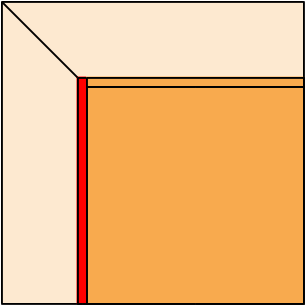
\includegraphics[width=0.8\linewidth]{linpack}}
      \only<2>{  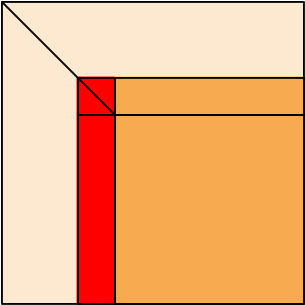
\includegraphics[width=0.8\linewidth]{lapack}}
      \only<3>{  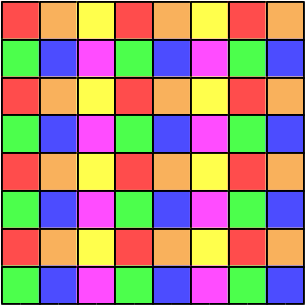
\includegraphics[width=0.8\linewidth]{scalapack}}
    \end{column}
  \end{columns}

\end{frame}

%\begin{frame}{Runtime Family}
%Runtime is a system which enable execution of a programme written in a specific language.
%
%For parallel distributed memory programs, we propose to distinguish runtimes to :
%
%\pause
%\begin{center}
%\begin{tiny}
%\begin{tabular}{|c|c|c|c|c|}
%\hline
%& \multicolumn{2}{c|}{Messaging Systems} & \multicolumn{2}{c|}{Task flow model} \\
%\hline
%Subfamily & Message passing & Active Message & Explicit Data Dependencies & Implicit Data Dependencies\\
%\hline
%Examples & MPI & Charm++ & Quarck, StarSS, \alert<3>{Starpu} & Intel CnC, \alert<3>{DAGuE} \\
%\hline
%\end{tabular}
%\end{tiny}
%\end{center}
%\end{frame}

%\begin{columns}[t]
%\begin{footnotesize}
%\begin{column}{.02\textwidth}
%\end{column}
%
%\begin{column}{.45\textwidth}
%\begin{exampleblock}{\centering Messaging Systems}
%\begin{columns}[onlywidth]
%\begin{column}{.45\textwidth}
%\centering
%Message passing\\
%MPI
%\end{column}\hfill
%\begin{column}{.45\textwidth}
%\centering
%Active message\\
%Charm++
%\end{column}
%\end{columns}
%\end{exampleblock}{}
%\end{column}
%
%\pause
%
%\begin{column}{.45\textwidth}
%\begin{exampleblock}{\centering Task flow model}
%\begin{columns}[onlywidth]
%\begin{column}{.02\textwidth}
%\end{column}
%\begin{column}{.45\textwidth}
%Explicit data dependencies\\
%StarSS, Quark, \alert<4>{StarPU}
%\end{column}\hfill
%\begin{column}{.45\textwidth}
%Implicit data dependencies\\
%Intel CnC, \alert<4>{DAGuE}
%\end{column}
%\end{columns}
%\end{exampleblock}{}
%\end{column}
%
%\end{footnotesize}
%\end{columns}
%\end{frame}

%\begin{frame}{Runtimes based on task flow model}
%\framesubtitle{Quick presentation}
%\begin{center}
%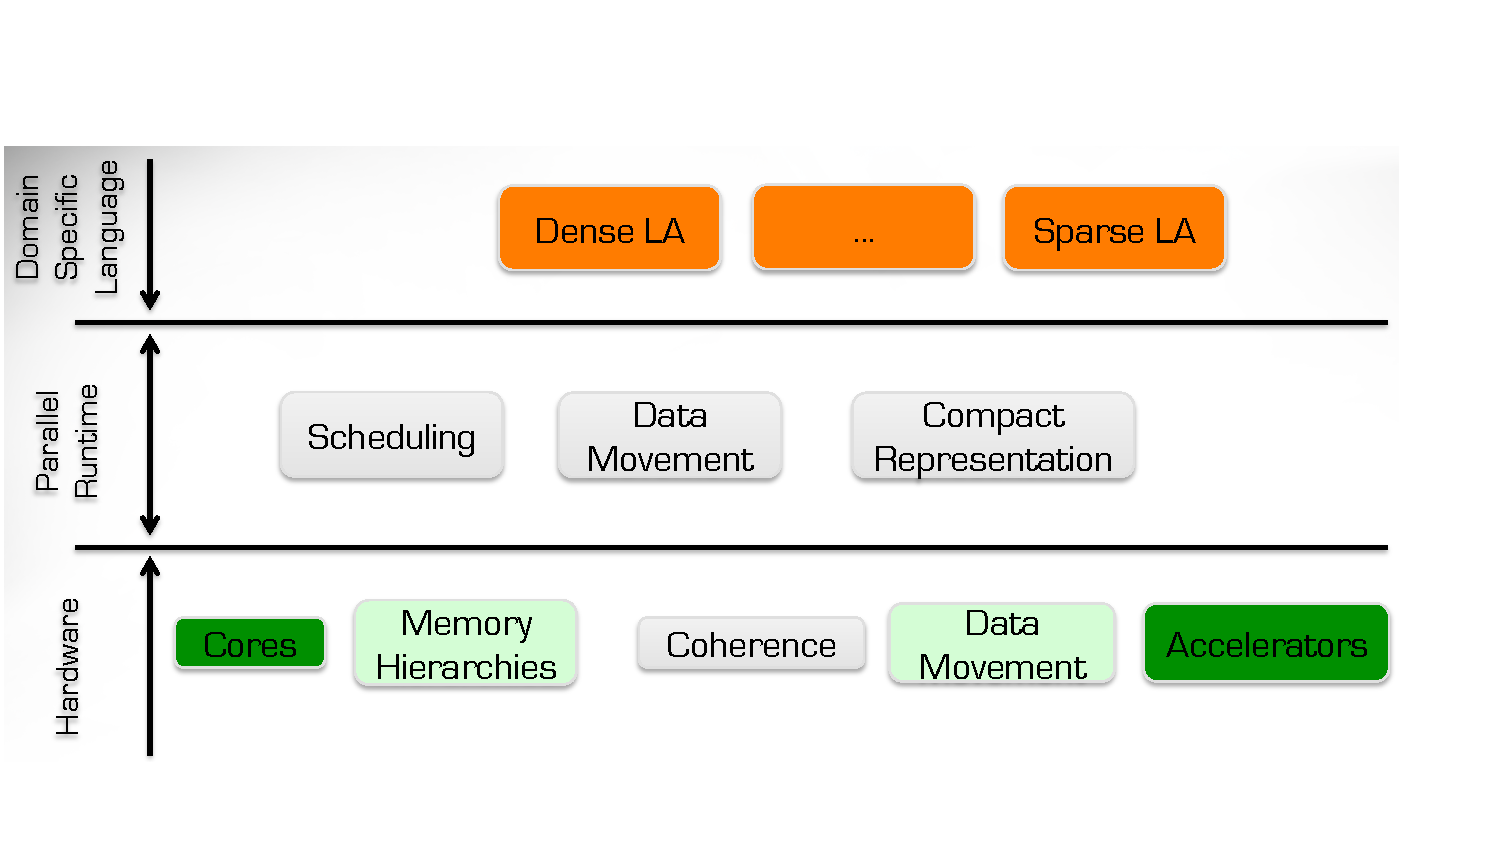
\includegraphics[scale=0.5]{3layer.pdf}
%\end{center}
%\end{frame}

%\begin{frame}{DAGuE}
%\framesubtitle{Quick presentation}
%DAGuE is a Direct Acyclic Graph scheduler Engine based on task flow model where :
%\begin{itemize}
%\item nodes are tasks
%\item edges are dependencies
%\end{itemize}
%\begin{center}
%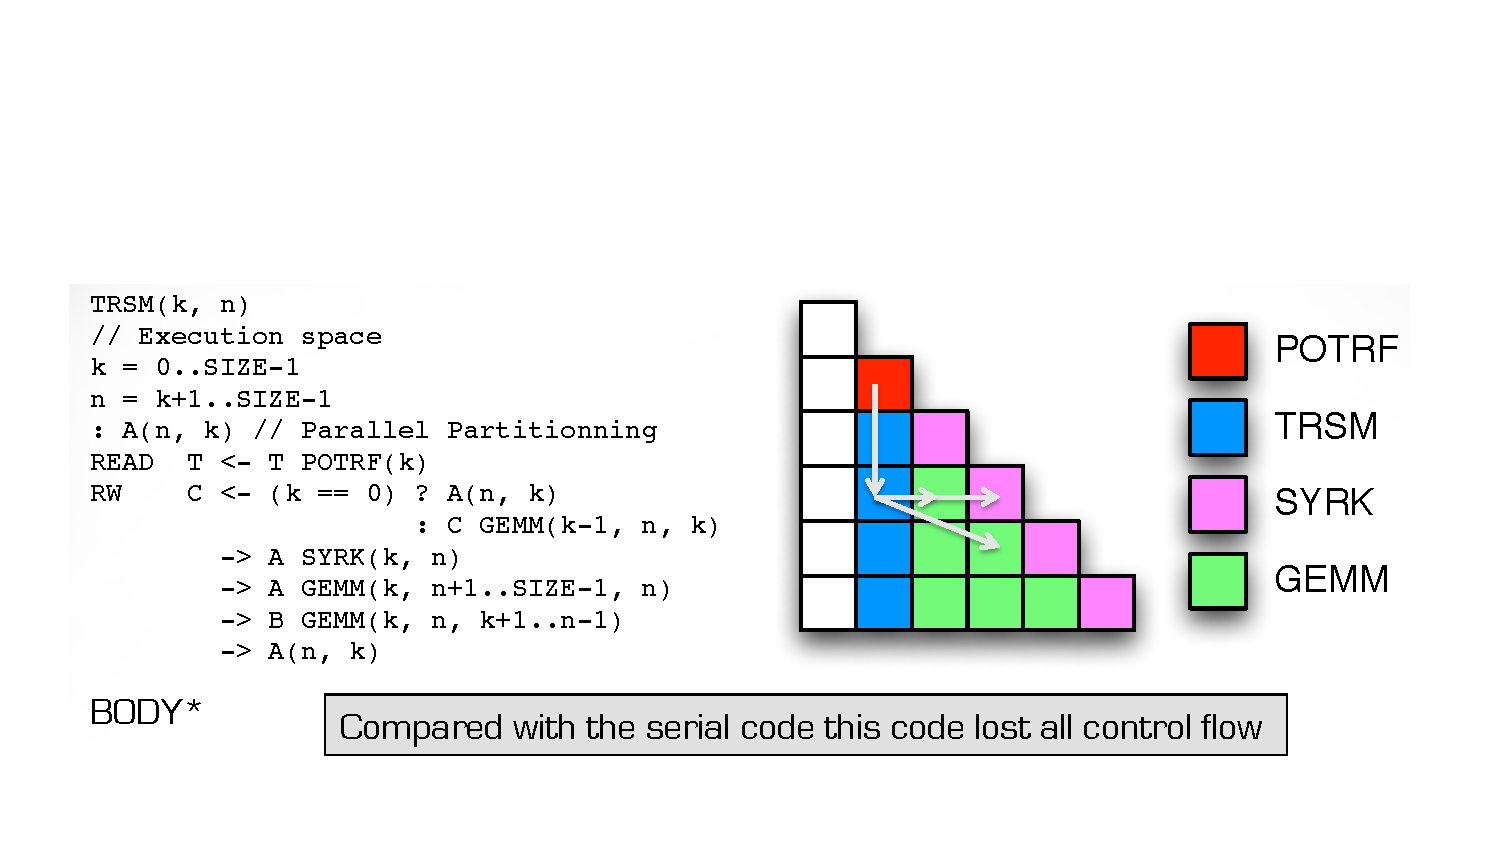
\includegraphics[scale=0.5]{trsm.pdf}
%\end{center}
%\end{frame}